\documentclass[10pt]{article}

\usepackage{ifthen}

%%%%
%% Begins the usepackage section
%%%%

\usepackage{amsmath}
\usepackage{amssymb}
\usepackage{amsthm}


%%
% slight detour to create the proper text/paper size.
% Depends on the ifthen package, needed before loading
% the geometry package
%%
\newboolean{sevenbytenbooksize}
\newboolean{ipadsize}   % for the ipad, Duh.
\newboolean{standard}

\setboolean{sevenbytenbooksize}{false}
\setboolean{ipadsize}{false}
\setboolean{standard}{true}
%
%	Note how the iPad version differs from the booksize only in 
% the size of the margins.
%
% Changing the following isn't hard but should be done with 
% practice and care, making sure to get the margins right for a 
% particular page size and printing format
%
%% Layout for printed book through Amazon CreateSpace, perfect bound,
%% 7x10 ``journal'' size

\ifthenelse{\boolean{ipadsize}}{\usepackage[paperheight=620pt,paperwidth=395pt, textheight=550pt,
textwidth=345pt, includeheadfoot, hcentering=true]{geometry}}{}

\ifthenelse{\boolean{sevenbytenbooksize}}{\usepackage[paperheight=10in,paperwidth=7in, textheight=550pt,
textwidth=345pt, inner=1in,includeheadfoot]{geometry}}{}

\ifthenelse{\boolean{standard}}{\usepackage{geometry}}{}

%% end detour
%%
\usepackage{layout}
\usepackage{graphicx}
\usepackage{multicol}
\usepackage{tikz}
\usetikzlibrary{calc}
\usepackage{makeidx}

\usepackage{changepage}
\usepackage{ulem}
\usepackage{xcolor}
\usepackage[bookmarksnumbered,linkbordercolor=white]{hyperref}

\usepackage{fancyhdr}
\usepackage{calc}

\makeindex

\newcommand{\apex}{A\kern -2pt \lower -2pt\hbox{P}\kern -4pt \lower .7ex\hbox{E}\kern -1pt X}


%%%%
%% The portions of the header containing fancyheader commands
%% has been moved to a book specific location and is not considered
%% part of the APEX header. This may change.
%%%%

%
%\pagestyle{fancy}
%\fancyhead{}
%\fancyfoot{}
%\renewcommand{\chaptermark}[1]{\markboth{\chaptername\ \thechapter\ \ \ \ {#1}}{}}
%\renewcommand{\sectionmark}[1]{\markright{\thesection\ \ \ \  #1}}
%\fancyhf{}         %Clears all header and footer fields, in preparation.
%
%\fancyhfoffset[LE,RO]{30pt}
%\fancyfoot[LE,RO]{\textbf{\thepage}} %Displays the page number in bold in the header,
%                       % to the left on even pages and to the right on odd pages.        
%\fancyhead[LE]{\nouppercase{\leftmark}}
%      %Displays the upper-level (chapter) information---
%      % as determined above---in non-upper case in the header, 
%      %to the right on even pages.
%\fancyhead[RO]{\rightmark}
%			%Displays the lower-level (section) information---as
%      % determined above---in the header, to the left on odd pages.
%\renewcommand{\headrulewidth}{0pt}
%\renewcommand{\footrulewidth}{0pt}
%	%Underlines the header and footer. (Set to 0pt if not required).


%%%%
%% Commands to determine whether we print in color or 
%% black and white
%%%%
\newboolean{in_color}

% determines the line colors for color and black and white lines.
\newcommand{\colorlinecolor}{blue!95!black!30}
\newcommand{\bwlinecolor}{black!30}

% sets the line color to be in color, as a default
\newcommand{\thelinecolor}{\colorlinecolor}

\newcommand{\setcolorlinecolor}[1]{\renewcommand{\colorlinecolor}{#1}\renewcommand{\thelinecolor}{\colorlinecolor}}
\newcommand{\setbwlinecolor}[1]{\renewcommand{\bwlinecolor}{#1}\renewcommand{\thelinecolor}{\bwlinecolor}}

% this allows the above default to be overriden by using
% the \printincolor and \printinblackandwhite commands
% anywhere in the file. This allows you to switch back
% and forth between bw and color. (Who would want to?)
\newcommand{\printincolor}{\setboolean{in_color}{true}%
\renewcommand{\thelinecolor}{\colorlinecolor}}
\newcommand{\printinblackandwhite}{\setboolean{in_color}{false}%
\renewcommand{\thelinecolor}{\bwlinecolor}}

% the default is printing in color
\printincolor

%% Creates a lot of measurements - lengths - to use
%% later on. Explained when a value is set.
\newlength{\topmarginlength} 
\newlength{\bottommarginlength}
\newlength{\oddpagemarginlength}
\newlength{\evenpagemarginlength}
\newlength{\marginlinelength}


% measures how far from the text the example line is to be drawn
\setlength{\marginlinelength}{5pt}

% the height of the top margin
% used in calculating the lines for examples
\setlength{\topmarginlength}{-1in-\voffset}

% the length of the bottom margin (ish)
% actually starts at the top of the page, moves
% through the top margin length then the text height.
\setlength{\bottommarginlength}{-1in-\textheight-2\baselineskip}

% the length of the left hand margin of an odd page
\setlength{\oddpagemarginlength}{1in+\hoffset+\oddsidemargin-2\marginlinelength}

% the length of the left hand margin of an even page
\setlength{\evenpagemarginlength}{1in+\hoffset+\evensidemargin-2\marginlinelength}


% creates a generic style for the lines. You can add lots
% of things here, all separated by commas.
\newcommand{\linestyle}{[thick, \thelinecolor]}

\newcommand{\setlinestyle}[1]{\renewcommand{\linestyle}{[#1, \thelinecolor]}}

% Do you want to draw the lines for examples? If so,
% use the first command. Otherwise, use the second. 
% The first is the default, but you can override it
% by using the second in your main file.
\newboolean{showexamplelines}
\newcommand{\drawexamplelines}{\setboolean{showexamplelines}{true}}
\newcommand{\nodrawexamplelines}{\setboolean{showexamplelines}{false}}

% by default the lines around the examples are drawn
\drawexamplelines


% This is more a debugging tool than a stylistic one.
% This draws a small circle in the margin at the the
% beginning of an example and another immediately follwing
% the end of the example, in the text. Sometimes it is useful
% to figure out why there seems to be a lot of space between
% the end of the example and the end of the drawn line.
% Too much space can occur, for instance, if the example ends with
% with a ``$$ maths $$'' type environment. You can correct for this
% with a \vskip -\baselineskip command.
\newboolean{showexamplemarks}
\newcommand{\drawexamplemarks}{\setboolean{showexamplemarks}{true}}
\newcommand{\nodrawexamplemarks}{\setboolean{showexamplemarks}{false}}
\nodrawexamplemarks

\newboolean{exampleisintext}
\newcommand{\exampleinmargin}{\setboolean{exampleisintext}{false}}
\newcommand{\exampleintext}{\setboolean{exampleisintext}{true}}
\exampleintext

\newcounter{examplecounter}
\setcounter{examplecounter}{0}

% the example environment has a regular and starred version.
% the regular version takes 3 arguments: label, problem, solution.
% The starred version only has 2: label, problem/solution.
\makeatletter
\newcommand{\example}{\@ifstar \examplestarred \examplenostar}
\newcommand{\reverseexampledefault}{\renewcommand{\example}{\@ifstar \examplenostar \examplestarred}}
\newcommand{\restoreexampledefault}{\renewcommand{\example}{\@ifstar \examplestarred \examplenostar}}
\makeatother

%% This is the no-star (regular) version of
%% the example command.
\newcommand{\examplenostar}[3]{%
%\ifthenelse{\boolean{in_color}}{renewcommand{\thelinecolor}{\colorlinecolor}}{\renewcommand{\thelinecolor}{\bwlinecolor}}%
\noindent%
\ifthenelse{\boolean{exampleisintext}}
{% default: the Example word is in text
\hskip -2\marginlinelength%
\parbox{\marginlinelength}{%
\begin{tikzpicture}[remember picture,overlay]%
\ifthenelse{\boolean{showexamplelines}}{\ifthenelse{\boolean{showexamplemarks}}
{\draw (0,0) circle (1pt) node (#1) {};}%
{\draw (0,0) node (#1) {};}
}
{}% ends the ``Draw example lines and marks?'' booleans
\end{tikzpicture}%
}% ends parbox where line begins
\hskip \marginlinelength% puts us back in line
\parbox{80pt}{{\bf Example \refstepcounter{examplecounter}\theexamplecounter}}% ends parbox
\label{#1}%
}% ends the if example in text; next do if not in text
{%
%\hskip -\marginlinelength%
\hskip -70pt%
\parbox{\marginlinelength}{%
\begin{tikzpicture}[remember picture,overlay]%
\ifthenelse{\boolean{showexamplelines}}{\ifthenelse{\boolean{showexamplemarks}}
{\draw (0,0) circle (1pt) node (#1) {};}%
{\draw (0,0) node (#1) {};}
}%
{}% ends the ``Draw example lines and marks?'' booleans
\end{tikzpicture}%
}%
\hskip -\marginlinelength
\parbox{70pt}{{\bf Example \refstepcounter{examplecounter}\theexamplecounter}}% ends parbox
\label{#1}%\hskip \marginlinelength%
}% ends if example in text
\ifthenelse{\pageref{#1}=\pageref{e#1}}% if the beginning and end are on the same page
{%
#2 \vskip \baselineskip%
\ifthenelse{\boolean{exampleisintext}}
{%solution is in text
\parbox{65pt}{\textsc{\small\bfseries Solution}}% 
}% solution is in margin
{\hskip -80pt%
\parbox{65pt}{\textsc{\small\bfseries Solution}}% 
\hskip 15pt%
}% end solution in margin
#3  \label{e#1}% writes the full example then draws the lines
\ifthenelse{\boolean{showexamplelines}}{%
\begin{tikzpicture}[remember picture,overlay]%
\ifthenelse{\boolean{showexamplemarks}}
{\draw (0,0) circle (1pt) node (e#1) {};}%
{\draw (0,0) node (e#1) {};}%
\ifthenelse{\boolean{exampleisintext}}
{\draw \linestyle (#1) -- (#1.south |- e#1.south) -- ++(10pt,0);}
{\draw \linestyle ([yshift=-3pt]#1.south) -- ++(70pt-2\marginlinelength,0) node (f#1) {} -- (f#1 |- e#1.south) -- ++(10pt,0);} 
\end{tikzpicture}
}{}% ends if/then/else show lines
}% ends if beginning and end are on same page.
% next is if they are on different pages
{% first draw line from start to bottom of page
\ifthenelse{\boolean{showexamplelines}}{%
\begin{tikzpicture}[remember picture,overlay]% 
\ifthenelse{\isodd{\pageref{#1}}}% draws lines based on whether on an even or odd page %
{\node [xshift=\oddpagemarginlength,yshift=\bottommarginlength](bottomleft) at (current page.north west)  {};}
{\node [xshift=\evenpagemarginlength,yshift=\bottommarginlength](bottomleft) at (current page.north west)  {};}
\ifthenelse{\boolean{exampleisintext}}% is example in text?
{\draw \linestyle (#1) -- (bottomleft);}
{\draw \linestyle ([yshift=-3pt]#1.south) -- ++(70pt-2\marginlinelength,0) --(bottomleft);} 
\end{tikzpicture}
}{}% ends if/then/else show lines
% end drawing of line
#2 \vskip \baselineskip%
\ifthenelse{\boolean{exampleisintext}}
{%solution is in text
\parbox{65pt}{\textsc{\small\bfseries Solution}}% 
}% solution is in margin
{\hskip -80pt%
\parbox{65pt}{\textsc{\small\bfseries Solution}}% 
\hskip 15pt%
}% end solution in margin
#3  \label{e#1}% now write out full example
% now draw line from end to top of page
\ifthenelse{\boolean{showexamplelines}}{%
\begin{tikzpicture}[remember picture,overlay] 
\ifthenelse{\boolean{showexamplemarks}}
{\draw (0,0) circle (1pt) node (e#1) {};}%
{\draw (0,0) node (e#1) {};}%
\ifthenelse{\isodd{\pageref{e#1}}}% draws lines based on whether on an even or odd page %
{\node [xshift=\oddpagemarginlength,yshift=\topmarginlength](topleft) at (current page.north west)  {};}
{\node [xshift=\evenpagemarginlength,yshift=\topmarginlength](topleft) at (current page.north west)  {};}
\draw \linestyle (topleft)--(e#1.south -| topleft) -- ++(10pt,0);
\end{tikzpicture}%
}{}% ends if/then/else show lines
}% ends the check for same page or not
%
}%ends the definition of example


\newcommand{\examplestarred}[2]{%
%\ifthenelse{\boolean{in_color}}{renewcommand{\thelinecolor}{\colorlinecolor}}{\renewcommand{\thelinecolor}{\bwlinecolor}}%
\noindent%
\ifthenelse{\boolean{exampleisintext}}
{% default: the Example word is in text
\hskip -2\marginlinelength%
\parbox{\marginlinelength}{%
\begin{tikzpicture}[remember picture,overlay]%
\ifthenelse{\boolean{showexamplelines}}{\ifthenelse{\boolean{showexamplemarks}}
{\draw (0,0) circle (1pt) node (#1) {};}%
{\draw (0,0) node (#1) {};}
}
{}% ends the ``Draw example lines and marks?'' booleans
\end{tikzpicture}%
}% ends parbox where line begins
\hskip \marginlinelength% puts us back in line
\parbox{80pt}{{\bf Example \refstepcounter{examplecounter}\theexamplecounter}}% ends parbox
\label{#1}%
}% ends the if example in text; next do if not in text
{%
%\hskip -\marginlinelength%
\hskip -70pt%
\parbox{\marginlinelength}{%
\begin{tikzpicture}[remember picture,overlay]%
\ifthenelse{\boolean{showexamplelines}}{\ifthenelse{\boolean{showexamplemarks}}
{\draw (0,0) circle (1pt) node (#1) {};}%
{\draw (0,0) node (#1) {};}
}%
{}% ends the ``Draw example lines and marks?'' booleans
\end{tikzpicture}%
}%
\hskip -\marginlinelength
\parbox{70pt}{{\bf Example \refstepcounter{examplecounter}\theexamplecounter}}% ends parbox
\label{#1}%\hskip \marginlinelength%
}% ends if example in text
\ifthenelse{\pageref{#1}=\pageref{e#1}}% if the beginning and end are on the same page
{%
#2 \label{e#1}% writes the full example then draws the lines
\ifthenelse{\boolean{showexamplelines}}{%
\begin{tikzpicture}[remember picture,overlay]%
\ifthenelse{\boolean{showexamplemarks}}
{\draw (0,0) circle (1pt) node (e#1) {};}%
{\draw (0,0) node (e#1) {};}%
\ifthenelse{\boolean{exampleisintext}}
{\draw \linestyle (#1) -- (#1.south |- e#1.south) -- ++(10pt,0);}
{\draw \linestyle ([yshift=-3pt]#1.south) -- ++(70pt-2\marginlinelength,0) node (f#1) {} -- (f#1 |- e#1.south) -- ++(10pt,0);} 
\end{tikzpicture}
}{}% ends if/then/else show lines
}% ends if beginning and end are on same page.
% next is if they are on different pages
{% first draw line from start to bottom of page
\ifthenelse{\boolean{showexamplelines}}{%
\begin{tikzpicture}[remember picture,overlay]% 
\ifthenelse{\isodd{\pageref{#1}}}% draws lines based on whether on an even or odd page %
{\node [xshift=\oddpagemarginlength,yshift=\bottommarginlength](bottomleft) at (current page.north west)  {};}
{\node [xshift=\evenpagemarginlength,yshift=\bottommarginlength](bottomleft) at (current page.north west)  {};}
\ifthenelse{\boolean{exampleisintext}}% is example in text?
{\draw \linestyle (#1) -- (bottomleft);}
{\draw \linestyle ([yshift=-3pt]#1.south) -- ++(70pt-2\marginlinelength,0) --(bottomleft);} 
\end{tikzpicture}
}{}% ends if/then/else show lines
% end drawing of line
#2 \label{e#1}% now write out full example
% now draw line from end to top of page
\ifthenelse{\boolean{showexamplelines}}{%
\begin{tikzpicture}[remember picture,overlay] 
\ifthenelse{\boolean{showexamplemarks}}
{\draw (0,0) circle (1pt) node (e#1) {};}%
{\draw (0,0) node (e#1) {};}%
\ifthenelse{\isodd{\pageref{e#1}}}% draws lines based on whether on an even or odd page %
{\node [xshift=\oddpagemarginlength,yshift=\topmarginlength](topleft) at (current page.north west)  {};}
{\node [xshift=\evenpagemarginlength,yshift=\topmarginlength](topleft) at (current page.north west)  {};}
\draw \linestyle (topleft)--(e#1.south -| topleft) -- ++(10pt,0);
\end{tikzpicture}%
}{}% ends if/then/else show lines
}% ends the check for same page or not
%
}%ends the definition of examplestarred

% Draws a line on a page that doesn't contain either
% the beginning or end of an example.
% Takes no arguments; figures out if you 
% are on an even or odd numbered page for
% correct margin calculation
\newcommand{\drawexampleline}{%
\begin{tikzpicture}[remember picture,overlay]
				\ifthenelse{\isodd{\thepage}}{%
				\node [xshift=\oddpagemarginlength,yshift=\topmarginlength](tleft) at (current page.north west)  {};}
				{\node [xshift=\evenpagemarginlength,yshift=\topmarginlength](tleft) at (current page.north west)  {};}
        \draw \linestyle (tleft) -- ++(0,-\textheight);
        \end{tikzpicture}
}


%
%Define style for Definitions, Theorems and Key Ideas  %%%%%%%%%%%%%%%%%%%%%%%%%%%%%%%%%%%%%%%%%%%%
%%%%%%%%%%%%%%%%%%%%%%%%%%%%%%%%%%%%%%%%%%%%%%%%%%%%%%%%%%%%%%%%%%%%%%%%%%%%%%%%%%%%%%%%%%%%%%%%%%%
%


\newlength{\specialboxlength}
\newlength{\specialboxtitlelength}
\newlength{\specialboxinnerseplength}

\setlength{\specialboxtitlelength}{75pt}
\setlength{\specialboxinnerseplength}{15pt}
\setlength{\specialboxlength}{\textwidth-\specialboxtitlelength-2\specialboxinnerseplength}


\long\def\newspecialbox#1#2#3#4{%
\newcounter{#1counter}
\expandafter\long\expandafter\def\csname #1\endcsname ##1##2{%
\vskip\baselineskip
\noindent\refstepcounter{#1counter}\label{##1}%
\begin{tikzpicture}
\draw (0,0) node[anchor=north west,text width=\specialboxtitlelength,inner sep=0pt]{\bf #2 \the\value{#1counter}};
\ifthenelse{\boolean{in_color}} %first, in color
{\draw (\specialboxtitlelength,0) node[rectangle,text width = \specialboxlength, inner sep=\specialboxinnerseplength, anchor=north west,yshift=\specialboxinnerseplength] [#3] {##2};}%if not in color
{\draw (\specialboxtitlelength,0) node[rectangle,text width = \specialboxlength, inner sep=\specialboxinnerseplength, anchor=north west,yshift=\specialboxinnerseplength]
 [#4] {##2};}
\end{tikzpicture}
}
}


\newspecialbox{definition}{Definition}{draw = yellow!95!black!60,top color = white!95!yellow,bottom color = yellow!90!black!30,text justified,very thick}{draw,text justified,very thick}

\newspecialbox{theorem}{Theorem}{draw = green!30!black!50,top color = white!95!green,bottom color = green!60!black!20, text justified,very thick}{draw,text justified,very thick}

\newspecialbox{idea}{Key Idea}{draw = red!30!black!50,top color = white!95!red,bottom color = red!60!black!20, text justified,very thick}{draw,text justified,very thick}


%%%%
%% Begins the exercise section, containing all commands
%% related to creating problem sections.
%%%%

\newcommand{\exc}{\addtocounter{excounter}{2}\arabic{excounter}}

\newif\ifmore

\newif\ifexsetmore

% this counter gives an effective, albeit not elegant
% way of using the same command to both print questions
% or the answers, depending on what section you are in.
% showexercises = 1: print questions
% showexercises = 2: print odd answers only
% showexercises = 3: print all answers 
% 
% The subsequent lines sets the value 
\newcount\showexercises
\newboolean{printquestions}
\newboolean{printoddanswersonly}

\setboolean{printoddanswersonly}{true}
\newcommand{\printallanswers}{\setboolean{printoddanswersonly}{false}}


\newcount\numberofexercises

\newcounter{numofexer}
\newcounter{negnumofexer}

% used for debugging; not really used anymore
\newcounter{debug}
\setcounter{debug}{0}

\newcounter{exercisecounter}
\newcounter{IMTcount}
\newcounter{IMTcount_temp}

% the exercise names can be printed next to the problem
% using these commands. The default is to not print them.
\newboolean{showexercisenames}
\newcommand{\printexercisenames}{\setboolean{showexercisenames}{true}}
\newcommand{\noprintexercisenames}{\setboolean{showexercisenames}{false}}
\noprintexercisenames


% TeX uses a certain system to name input files that it reads from.
% To prevent conflicts, we use the newread command.
\newread\exread %read an example
\newread\exsetread %read an example set
\newread\exansread %read the answer
\newread\printansread% read in the answers file

\newwrite\answrite %write the answers file
% give the answers file the name ``jobname.answers''
\openout\answrite=\jobname.answers

\def\exinput #1 {\ifthenelse{\boolean{printquestions}}{% 
												\openin\exread=#1 
												\read\exread to \tempp 
												\begin{enumerate} 
													\addtocounter{enumi}{\theexercisecounter}
													\item 
													\ifthenelse{\boolean{showexercisenames}}
													{\tiny {\hskip -60pt}% This line too
												  \makebox[60pt][l]{\printexercisename #1 }%  
												  \small%
												  }{}
													\tempp 
													\addtocounter{exercisecounter}{1}
												\end{enumerate}
												\closein\exread}% end print questions 
									{% else: print answers
									\ifthenelse{\boolean{printoddanswersonly}}{%i.e, we are printing odd answers, not questions 
												\openin\exread=#1 
												\read\exread to \tempp % read in the question - we ignore it.
												\addtocounter{exercisecounter}{1}
												\read\exread to \tempp % reads in the answer
												\ifodd \theexercisecounter
												%\else
													\begin{enumerate} 
													\addtocounter{enumi}{\theexercisecounter}
													\addtocounter{enumi}{-1}
													\item 
													\ifthenelse{\boolean{showexercisenames}}
													{\tiny {\hskip -60pt}% This line too
												  \makebox[60pt][l]{\printexercisename #1 }%
												  \small%
												  }{}
													\tempp 
													%\addtocounter{exercisecounter}{1}
													\end{enumerate} 
												\fi
												\closein\exread 
												}  %ends the \ifnum \showexercises = 2 if statement
												{% print all answers
												\openin\exread=#1 
												\read\exread to \tempp %reads in the question, which is ignored 
												\read\exread to \tempp %reads in the answer
												\begin{enumerate} 
													\addtocounter{enumi}{\theexercisecounter}
													\item 
													\ifthenelse{\boolean{showexercisenames}}
													{\tiny {\hskip -60pt}% This line too
												  \makebox[60pt][l]{\printexercisename #1 }%
												  \small%
												  }{}
													\tempp 
													\addtocounter{exercisecounter}{1}
												\end{enumerate}
												\closein\exread
												} % ends the \ifnum \showexercises=3 if statement
									}
								}

\def\exsetinput #1 {\openin\exsetread=#1
										\setcounter{numofexer}{0}
										\setcounter{negnumofexer}{0} 
										\read\exsetread to \exsettemp
										\read\exsetread to \exsettemp
										{\loop
												\read\exsetread to \exsettemp
												\ifeof \exsetread \exsetmorefalse \else \exsetmoretrue \fi
												\ifexsetmore
														\addtocounter{numofexer}{1}
														\addtocounter{negnumofexer}{-1}
											\repeat}							
										\closein\exsetread
										\openin\exsetread=#1
										\ifthenelse{\boolean{printquestions}}{ 
											\read\exsetread to \exsettemp
											\setcounter{enumi}{\theexercisecounter} 
											\addtocounter{enumi}{1}
											\ifthenelse{\boolean{showexercisenames}}
													{\tiny {\hskip -60pt}% This line too
												  \makebox[60pt][l]{\printexercisename #1 }%
												  \small%
												  }{}% end show exercise names
											\noin\textbf{\exsettemp\theenumi\addtocounter{enumi}{-1}
											\addtocounter{enumi}{\thenumofexer}{-- }\theenumi%
											\addtocounter{enumi}{\thenegnumofexer}%
											\read\exsetread to \exsettemp \exsettemp}%
											
											{\loop
													\read\exsetread to \exsettemp
													\ifeof \exsetread \exsetmorefalse \else \exsetmoretrue \fi
													\ifexsetmore
															\exsettemp
											\repeat}
										}% ends print exercises; on to print answers
										{	\read\exsetread to \exsettemp
											\read\exsetread to \exsettemp
											{\loop
													\read\exsetread to \exsettemp
													\ifeof \exsetread \exsetmorefalse \else \exsetmoretrue \fi
													\ifexsetmore
															\exsettemp
											\repeat}
										}%ends else printing asnwers
										\closein\exsetread
								}

\def\printexercises #1 {%
\ifthenelse{\equal{\expandafter\readsection\thesection}{1}}{\immediate\write\answrite{\noexpand \noindent {\noexpand\Large\noexpand\bf Chapter \thechapter} \noexpand \vskip \noexpand\baselineskip } \write\answrite{}}{}%
\immediate\write\answrite{\noexpand\noindent {\noexpand\bf Section \thesection} \noexpand \vskip \baselineskip}%
\write\answrite{\noexpand\printanswers{#1}}%
\setcounter{exercisecounter}{0}\setboolean{printquestions}{true} \small%
\noin\underline{\parbox{\textwidth}{\Large\textbf{Exercises \thesection} }}% 
\sffamily%
\vskip\baselineskip%
\begin{multicols}{2}%
				\openin\exansread=#1 
				\ifeof \exansread 
					{No problems written.} 
				\else 
					\loop \read\exansread to \extemp  
							\ifeof \exansread \morefalse \else \moretrue \fi 
							\ifmore 
									\extemp
							\repeat 
				\fi 
				\closein\exansread 
				\end{multicols}%
				\setlength{\hoffset}{0pt} \rmfamily\normalsize \vskip \baselineskip%
				}
				


% The following prints the answers. To print all answers, use command \printallanswers.
% 
\def\printanswers #1 {\setcounter{exercisecounter}{0} \footnotesize \setboolean{printquestions}{false} \openin\printansread=#1 
				\ifeof \printansread 
					{No problems written.} 
				\else 
					\loop \read\printansread to \extemp  
							\ifeof \printansread \morefalse \else \moretrue \fi 
							\ifmore 
									\extemp
							\fi 
							\ifeof \printansread \morefalse \else \moretrue \fi 
							\ifmore 
					\repeat 
				\fi 
				\closein\printansread
				\small}

								
\def \printexercisename exercises/#1_#2_#3_#4 {#1 #2 #3 #4}

%%%%%%%%%%%%% Used to automate the answer production at
%%%%%%%%%%%%% end the text.

\def \readsection #1.#2{#2}

\def \writeexercisestofile #1{%
\write\answrite{\noexpand\printanswers{exercises/0\thechapter_0\expandafter\readsection #1_exercises.tex} \noexpand \vskip \baselineskip } \write\answrite{} }

\def \makeexercisesection #1{\write\answrite{\noexpand\end{multicols}
\noexpand\normalsize} \closeout\answrite \chapter{#1} \input{\jobname.answers}}%

%
% The following is a line of code, not a definition. 
% It writes the first line of the ``.answers'' file
% to set up the proper formatting of that file.
%
\write\answrite{\noexpand\small\noexpand\raggedright\noexpand\begin{multicols}{2}}


%\usepackage{underscore}
\usepackage{lipsum}
\usepackage{pdfpages}

\begin{document}

\begin{center} \Large {\bf APEX Formatting Guide}

\small
\tableofcontents
 \normalsize \end{center}
 
\section{Introduction} 

This manual is intended to guide the user through using a set of macros designed to facilitate the writing of mathematics texts. There are four main sections to this document: writing exercise/answer sections, an environment for writing examples within the text, environments for writing definition/theorem statements (and the like), and a section that highlights some other commands pertinent throughout.

\section{Writing Exercises}

One could ``easily'' write exercises for a mathematics text by creating an Enumeration environment and writing each problem as a new \verb|\item|. However, this can be cumbersome for a variety of reasons. Without highlighting the difficulties of this method, we posit the following system obviously takes greater initial effort but with overall positive gain. If one disagrees, feel free to use \verb|\begin{enumerate}|. 

A fundamental principle to the APEX format is that each exercise is contained in its own file that consists of two lines. The first line contains the problem statement; the second contains the answer (of course, the content level of the answer is up to the author). Instead of writing problems/answers in a cumbersome fashion to maintain the two line rule, it is much more convenient to enclose the problem and solution each in a set of curly braces, \verb|{ }|. So a sample exercise might consist solely of the following:
\begin{verbatim}
{Evaluate the following definite integral: 
$\int_0^1 x^2\ dx$.}
{$\frac13$}
\end{verbatim}

Naming this file properly is important. While the following restrictions may someday be removed, for now it is necessary to name the exercise file with the following convention: {\it chapnum\_secnum\_{\rm ex}\_probnum.{\rm tex}}. So the seventeenth problem you've written for chapter 3, section 5 would be named \verb|03_05_ex_17.tex|. Of course, this might not end up being the seventeenth problem of that section, nor must it end up in that section. It is helpful as you write to number your exercises for the section you intend them to end up in; later on, it won't matter what their actual name is.

As one's text grows in size, one will have written \textit{many} exercises, likely over an extended period of time. If one wants to edit the problem in section 4 of chapter 3, one is likely to have forgotten what that actual problem is named. To facilitate finding the name of the problem, one can include the command \verb|\printexercisenames| in the text. All subsequent exercise names will be printed unless the command \verb|\noprintexercisenames| is given. Of course, by default, exercise names are not printed. Make note: printing the names changes the format of the page slightly. Do not try to make final formatting changes to the document while exercise names are shown.

To actually create an exercise section, create a file that contains the names of the exercises to be included in the following fashion. One can name this file in whatever manner they please, but it makes common sense to name is something like \verb|01_05_exercises.tex| for the exercises for chapter 1, section 5. 

This exercise file will contain a series of one line commands, all either \verb|\exinput| or \verb|\exsetinput| commands. The \verb|\exsetinput| command will be explained shortly. A typical exercise file will look something like:
\begin{verbatim}
\exset{01_01_ex_01}
\exset{01_01_ex_02}
\exset{01_01_ex_04}
\exset{01_01_ex_03}
\end{verbatim}

The exercise file is effectively read twice in the printing of the document. The first time it is read it is used to create the exercise section. It is read again to produce the answer section. Therefore the \verb|\exset| command pulls double duty, either giving commands to print the question or the answer.

To actually produce the exercise section (likely at the end of the current section), use the command \verb|\printexercises|, as in \par \verb|\printexercises{01_01_exercises}|. This command does many things. It first prints the word ``Exercises'' followed by the current section. All of this is followed by a horizontal rule that extends the width of the text. Then the exercises are printed in two column format, in the \verb|\small| text size. These formatting settings are not too difficult to change; one can delve into the appropriate section of the file \verb|Header_APEX.tex| and make changes.

This setup produces a perfectly serviceable exercise section. However, many times one wants to give students practice by giving multiple problems with the same basic instructions. Instead of writing 
\begin{verbatim}
1. Find the derivative of $f(x) = x^2$.
2. Find the derivative of $f(x) = 2x^3$.
3. Find the derivative of $f(x) = \cos x$.
\end{verbatim}
one could just write the instructions once, as in 
\begin{verbatim}
In Exercises 1 - 3, find the derivative of the given function.

1. $f(x) = x^2$.
2. $f(x) = 2x^3$.
3. $f(x) = \cos x$.
\end{verbatim}

This type of construction is referred to as an ``exercise set.'' To create an exercise set, one first creates individual problems to be included in the set. This is done in the same fashion as before. Using our example above, problem 1 could be created with the following two lines:
\begin{verbatim}
{$f(x) = x^2$}
{$f'(x) = 2x$}
\end{verbatim}
Note that the actual problem statement does not appear here.

An exercise set file is now created. It consists of the statement of the problem in two parts, followed by a listing of the problems that are to be included in this exercise set.

The macros will automatically determine the numbering to be used in the statement of the problem for the set. The two part statement of the problem consists of the wording before the problem range (enclosed in curly braces), followed by the the wording following the problem range, also enclosed in curly braces. Again, as an example, consider the sample exercise set given above. The corresponding set file would look like
\begin{verbatim}
{\noindent In Exercises}
{, find the derivative of the given function.}
\exinput{01_01_ex_01}
\exinput{01_01_ex_02}
\exinput{01_01_ex_03}
\end{verbatim}

The APEX macros automatically figure out the numbering and place it immediately following the ``Exercises'' and preceding the ``\ ,\ ''. Note that in this example the command \verb|\noindent| is used; that is purely preferential. 

In creating exercise set files, care should be taken that no extra lines appear at the end of the file. The problem numbering range is determined by reading the number of lines in the exercise set file; extra lines at the end, even if blank, will give incorrect numbering.

Name this exercise set using the convention used before; the first exercise set one writes in section 7 of chapter 2 could be named \verb|02_07_exset_01|. 

To include this exercise set along with all other exercises, in the main exercise file use the command \verb|\exsetinput|, as in \verb|\exsetinput{02_07_exset_01}|.

A complete exercise file that could be used to produce the exercises for a section could look like the following, taken from an actual textbook.

\begin{verbatim}
\exsetinput{exercises/01_01_exset_01}
\exsetinput{exercises/01_01_exset_02}
\exinput{exercises/01_01_ex_19}
\exinput{exercises/01_01_ex_21}
\end{verbatim}

While it is not evident here, there are a total of 16 exercises in this section. The first exercise set contains 10 problems, the second 4, followed by two individual problems. 

\section{An Environment For Creating Examples}

\subsection{Basic Principles}
Examples are an important part of many textbooks. It is often useful to number these examples so that they can be referenced later on, and certainly one does not want to keep track of such numbering on their own. It is also useful to have a consistent way of signifying that an example is over. There is of course no ``right'' method of doing this and is subject to personal opinion. The APEX format file gives two ways of accomplishing this that look nice. Each method starts an example with the word {\bf Example} followed by a number; the example text is matched by a line drawn in the margin. The default method puts the word {\bf Example} in line with the text, while optionally one can put {\bf Example} in the margin to help distinguish it. At the moment, the ability to modify these is restricted by the user's ability to write \LaTeX\ code; simple modifications are likely not simple to implement, and complicated changes are probably $\ldots$ complicated. A sample example is shown further on in this section.

There are two basic forms of the example environment. The standard, \verb|\example|, takes three arguments. The first is a label for the example that can be used later for reference purposes (using the \verb|\ref| or \verb|\pageref| commands). The second argument is the statement of the problem the example is designed to solve. The third argument is the solution to the problem. The word \textsc{\small\bfseries Solution} appears indented on the left at the beginning of the solution, placed there by the macro.

An alternate example environment uses the \verb|\example*| command, which takes two arguments. The first is again the label; the second is the complete text of the example. This is used for examples that do not fit the ``State a problem then show the solution'' model. It does not print the word \textsc{\small\bfseries Solution}.

If one is pleased with the general output of the default settings, one's final concern is the label used in the first argument. It is the convention of many to use a label such as \verb|ex:01| to denote that this is the first example (whereas the first theorem might be labeled with \verb|thm:01|). However, due to the internal workings of the macro, the colon ``\verb| : |'' \textit{cannot} be used. It is suggested that the underscore \verb|_| be used instead, as in \verb|ex_01|. 

An example is given below.\\


\example{ex_first_example}{How does one go about creating an example? Show in just a few easy steps.}{Creating an example is easy. For instance, this example was created with the {\tt $\backslash$example} command. The first argument, the label, is {\tt ex\textunderscore first\textunderscore example.} 
The second argument, enclosed in curly braces, starts with \texttt{\{How does one.}$\ldots$ and ends with $\ldots$\texttt{easy steps.\}} 
The third argument is the solution, which starts with \texttt{\{Creating an example}$\ldots$ and ends with $\ldots$\texttt{self referencing.\}}
, highlighting the computer scientist's penchant for self referencing.}

\subsection{Options}

There are several options available in adjusting the look of examples. After describing the changes we offer several pages of examples.

\begin{description}
\item [In Margin / In Text]
It was previously mentioned that the APEX format allows one to put the word {\bf Example} either in the text or in the margin. One can switch between the two by using the commands \verb|\exampleintext| and \verb|\exampleinmargin|. They can be used anytime within the text and all subsequent examples will be typeset accordingly until the alternate command is given.

\item	[Line Options] There are several parameters concerning the lines that are drawn that can be adjusted.

	\begin{description}
	\item	[Drawing Lines] 
One can choose to not draw lines. One may be interested in doing this during the proof reading stages of the text. For reasons we'll leave unexplained, it can take as many as three compilations before the lines appear in the correct places. In the meantime, the lines may appear in odd and distracting places. By default, the lines are drawn. To turn them off, use the command \verb|\nodrawexamplelines| and all subsequent lines will be drawn. To turn them back on, use \verb|\drawexamplelines|.
	\end{description}
One can also format the style of the line. It may help to know some Ti{\it k}Z and \verb|xcolor| commands here. The default format is to draw a \verb|thick| line with color \verb|blue!95!black!30|. This can be changed.
		\begin{description}
		\item [Color] One can choose to print in black and white. This is especially good for when a printed copy is to be made, as black and white printed copies of color generally don't turn out quite right. To print in black and white, use the command \verb|\printinblackandwhite|. The default black and white color is a gray-scale color, namely \verb|black!30|. To go back to color, use \verb|\printincolor|. \\
		
		One may change these colors. To change the color color, use the command \verb|\setcolorlinecolor{|{\it color}\verb|}|. One may use the standard \verb|xcolor| options, such as \verb|red|, \verb|blue|, \verb|green| or use mixtures as shown above. Use Google to learn more about how to mix the color.\\
		
		To change the black and white color, use the command 
		
		\verb|\setbwlinecolor{|{\it color}\verb|}|. This color doesn't have to be ``black and white;'' one can make it \verb|green| if you like. \\
		
		Note: when using either of the above options, not only is that color set, it becomes the default option. So if you set the color color but want to continue printing in black and white, you need to follow with the \verb|printinblackandwhite| command.
		
		\item [Line Style] The style of the line can also be determined. To set this, use the \verb|\setlinestyle{|{\it options}\verb|}| command. The {\it options} can be any comma-delimited list of Ti{\it k}Z path options such as \verb|thin|, \verb|ultra thick|, \verb|dashed| or even \verb|->| to draw arrows. See the Ti{\it k}Z manual for more options. Note: while you are able to include a color within this list, it will likely not take effect. Set the color using the options above. 
		
		\item [Help Marks] The \verb|\drawexamplemarks| command draws a small circle at the beginning of the example line and at the end of what it considers to be the end of the example. This can be useful in ``debugging'' the results of an example. Sometimes extra space is added to the end of example, especially if the example ends with the end of an environment. (I.e., you end the example with an enumerated list or some mathematics inside of \verb|$$ ... $$|.) In such cases, a vertical skip of \verb|\baselineskip| is added, which causes the example line to end seemingly far below the actual end of the example. In such a case, it can help to have a small circle drawn to show where \LaTeX\ thinks the example ends. In the above cases, the extra space can be removed using the command \verb|\vskip -\baselineskip|. More/less space can be removed by adding a coefficient in front of the \verb|\baselineskip|. \\
		
		Sometimes the example ends on a following page, even though all the text ends on the previous page. The culprit is likely and extra \verb|\baselineskip|, but sometimes the trouble is harder to diagnose. Try enlarging the current page with \verb|\enlargethispage\baselineskip| or \verb|\enlargethispage2\baselineskip|, etc., to make the current page larger hence allowing the example to end without starting a new page.
		\end{description}
\end{description}


\theorem{thm:1}{This is a new theorem}

\newspecialbox{greg}{Gregory}

\greg{g1}{New definition?}

\greg{g2}{help}

\setlength{\specialboxtitlelength}{100pt}

\newspecialbox{ggreg}{HartmanHartman}

\ggreg{g3}{New box}

\ggreg{r5}{Hallow!}


See HartmanHartman \ref{r5}


%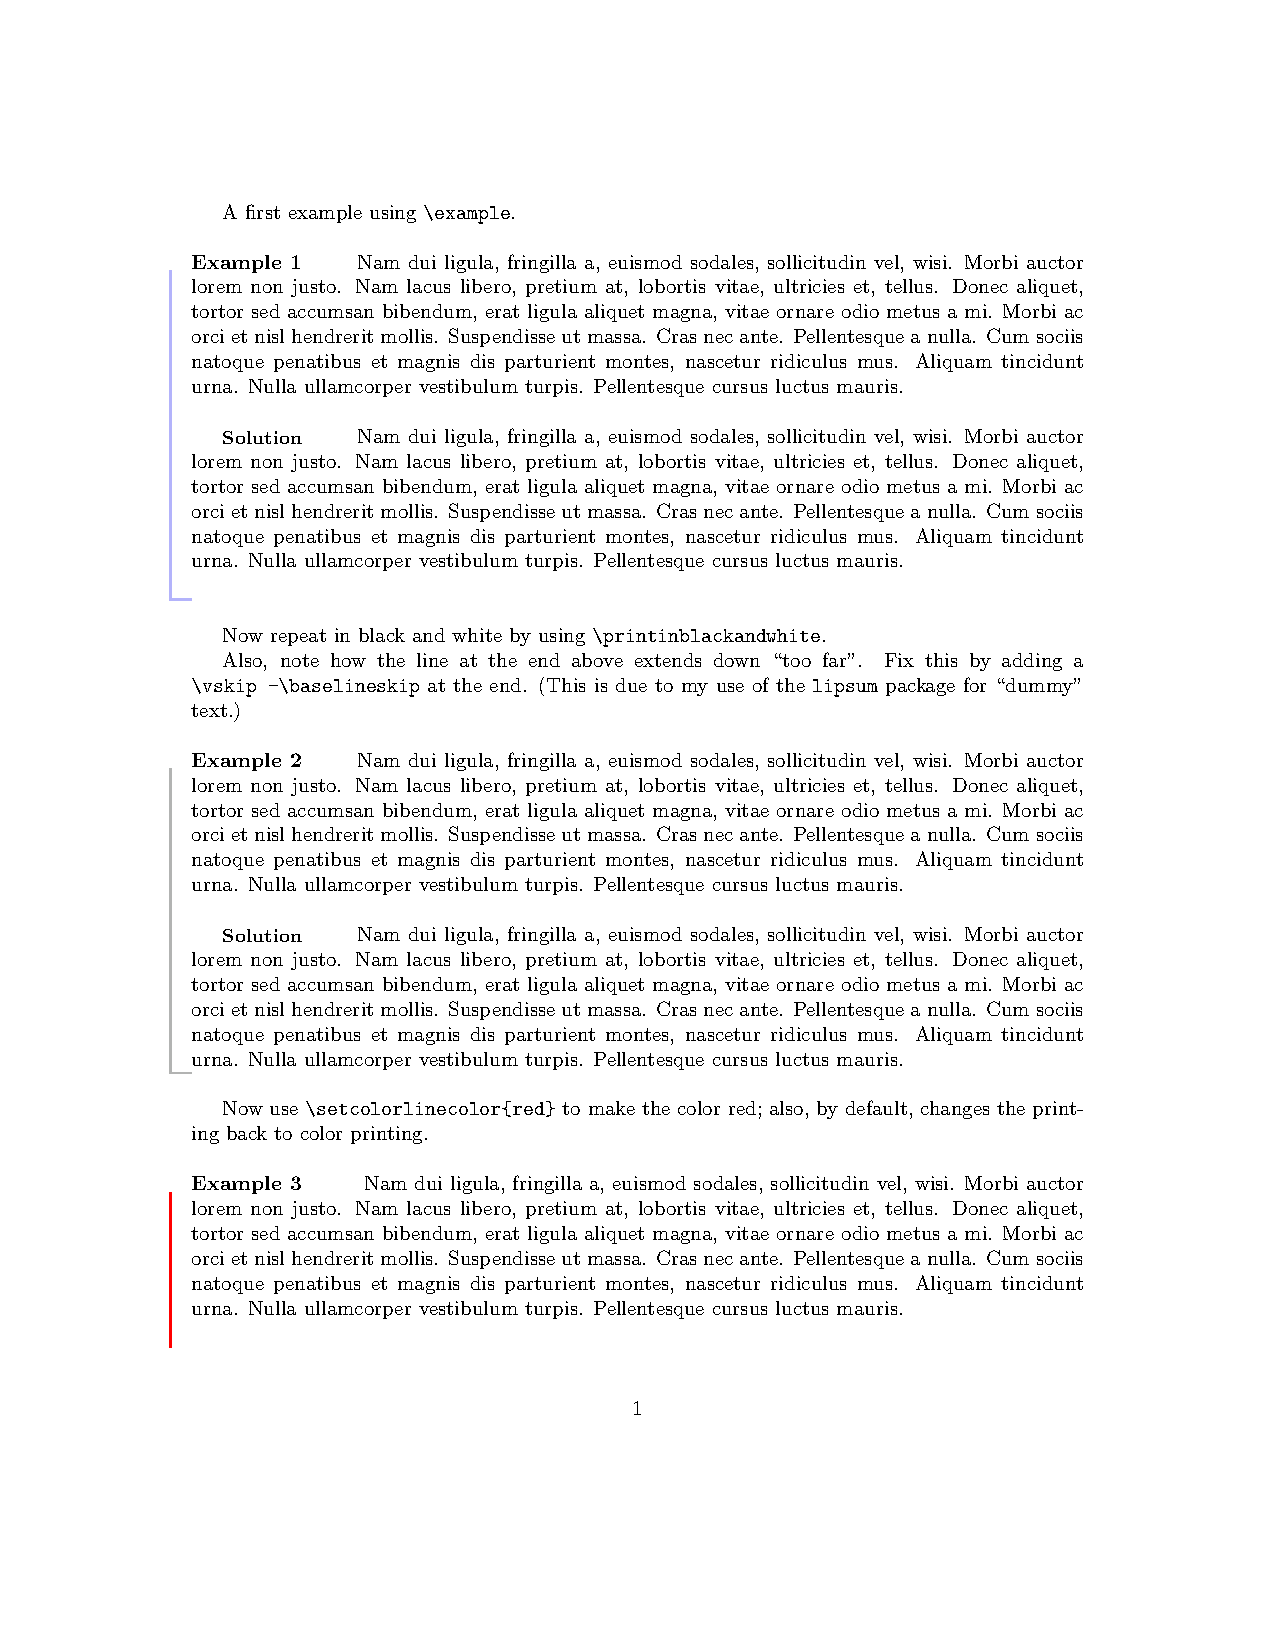
\includepdf[pages={1-2},nup=1x2,landscape=true]{APEX_Format_Examples}



%
%\printinblackandwhite
%
%\example{ex_second}{\lipsum[1]}{\lipsum[2]  \vskip -\baselineskip}\\
%
%\setcolorlinecolor{red}
%\example{ex_third}{\lipsum[1]}{\lipsum[1-2]}
%\setlinestyle{thin,dashed}
%
%\example*{ex_fourth}{\lipsum[1]}

\end{document}